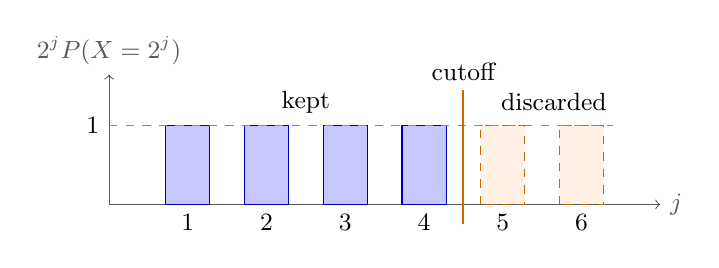
\begin{tikzpicture}[x=1.0cm,y=1cm]
\draw[->,black!65] (0,0)--(7,0) node[right,font=\small] {$j$};
\draw[->,black!65] (0,0)--(0,1.65) node[above,font=\small] {$2^jP(X=2^j)$};
\foreach \j in {1,2,3,4}{
  \draw[fill=blue!22,draw=blue!70!black] (\j-0.28,0) rectangle (\j+0.28,1);
}
\foreach \j in {5,6}{
  \draw[dashed,fill=orange!10,draw=orange!80!black] (\j-0.28,0) rectangle (\j+0.28,1);
}
\foreach \j in {1,2,3,4,5,6}{\node[below,font=\small] at (\j,0) {$\j$};}
\draw[dashed,black!45] (0,1)--(6.4,1);
\node[left,font=\small] at (0,1) {$1$};
\draw[thick,orange!80!black] (4.5,-0.25)--(4.5,1.45);
\node[above,font=\small] at (4.5,1.45) {cutoff};
\node[font=\small] at (2.5,1.3) {kept};
\node[font=\small] at (5.65,1.3) {discarded};
\end{tikzpicture}
